\documentclass[a4paper]{article}
\usepackage{cmap}
\usepackage{mathtext}
\usepackage{amssymb}
\usepackage{amsmath}
\usepackage[russian]{babel}
\usepackage{indentfirst}
\usepackage[pdftex]{graphicx}
\usepackage{multirow}
\usepackage{mathrsfs}
\usepackage{biblatex}
\usepackage{siunitx}
\usepackage[left=2cm,right=2cm,top=2cm,bottom=2cm]{geometry}
\usepackage{fancyhdr}
\bibliography{bib}
\pagestyle{fancy}
\newcommand{\rref}[1]{(\ref{#1})}
\newenvironment{comment}{}{}
\newcommand{\picref}[1]{рис. \ref{#1}}
\newcommand{\mbf}{\mathbf}
\newcommand{\Equip}[3]{
	
	{\bf #1:} $\Delta = \pm #2$ \si{#3}}
\newcommand{\equip}[1]{
	
	{\bf #1}}
\newcommand{\labname}{Изучение центрированных оптических систем} 	% название пиши здесь
\newcommand{\labnum}{4.1.1}		% номер вводи здесь
\fancyfoot{}
\fancyhead[RE, RO]{\thepage}
\fancyhead[LE, LO]{Лабораторная работа \labnum \space \labname}
\title{Лабораторная работа \labnum \space \labname} % Название работы здесь
\author{Иван Сладков}
\begin{document}
\maketitle
\thispagestyle{empty}
\section{Аннотация}
В данной работе проводится изучение методов определения фокусных расстояний линз и сложных оптических систем, а также определение характеристик оптической системы, составленной из тонких линз; производится изучение недостатков реальных линз — сферической и хроматической аберраций.


\section{Теоретические сведения}

\begin{figure}[tbp]
	\centering
	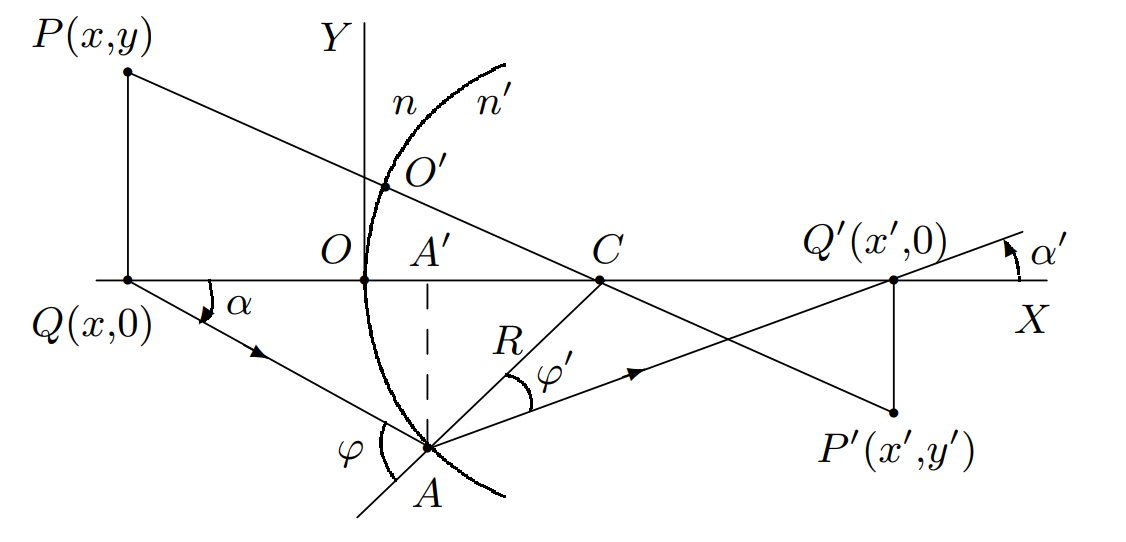
\includegraphics[width=0.8\linewidth]{Screenshot_1}
	\caption{Элементарная оптическая ячейка}
	\label{2}
\end{figure}


Используя закон преломления, получим для элементарной оптической ячейки, изображённой на \picref{2}, в параксиальном приближении:
\begin{equation}\label{опт-ячейка}
	-\frac{n}{x}+\frac{n'}{x'} = \frac{n'-n}{R},
\end{equation}
\begin{equation}
	x \alpha = x' \alpha'.
\end{equation}
Для прямой $ P P' $, рассмотренной как оптическая ось, 
\begin{equation}\label{PP}
	\frac{y'}{y} = \frac{x' - R}{x - R}.
\end{equation}

Проведя замену переменных, получим систему уравнений
\begin{equation}\label{grid}
	\frac{x' - F'}{H' - F'}= \frac{H-F}{x- F} = \frac{y'}{y} = \frac{n \alpha}{n' \alpha'},
\end{equation}
\begin{equation}\label{grid1}
	(x-H)\alpha= (x' - H')\alpha'.
\end{equation}
Из этих уравнений получим
\begin{equation}\label{Ф}
	\frac{n}{f} = -\frac{n'}{f'} \equiv \Phi,
\end{equation}
где
\begin{equation}\label{focus-len}
	f\equiv H - F, \;\;\; f'\equiv H' - F'.
\end{equation}
$ f $ и $ f' $ -- главные фокусные расстояния системы.





\subsection{Определение фокусного расстояния тонкой собирающей линзы и сложных оптических систем по методу Аббе}

Схема, применяемая для определения фокусного расстояния $ F $ оптической системы по методу Аббе, изображена на \picref{1}.
\begin{figure}[tbp]
	\centering
	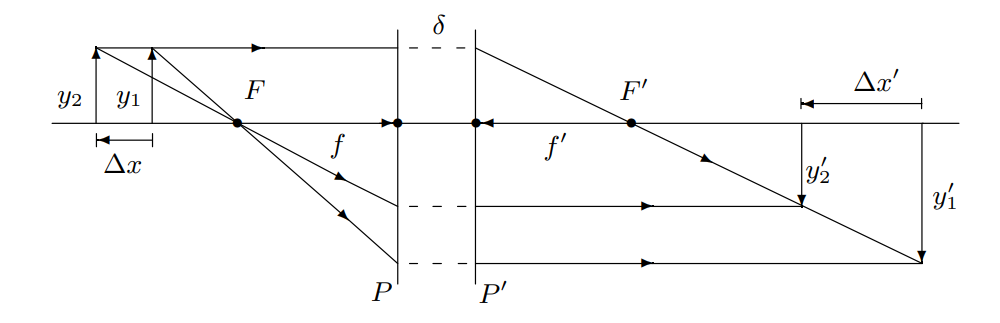
\includegraphics[width=0.8\linewidth]{Screenshot_3}
	\caption{Иллюстрация метода Аббе}
	\label{1}
\end{figure}

Из формул \eqref{Ф}, \eqref{grid}, \eqref{focus-len} получим:
\begin{equation}\label{abbe}
	f = \frac{\Delta x}{\Delta (y/y')} = -\frac{\Delta x'}{\Delta (y'/y)}.
\end{equation}

\subsection{Определение фокусного расстояния собирающих линз и сложных оптических систем по методу Бесселя}

\begin{figure}[tbp]
	\centering
	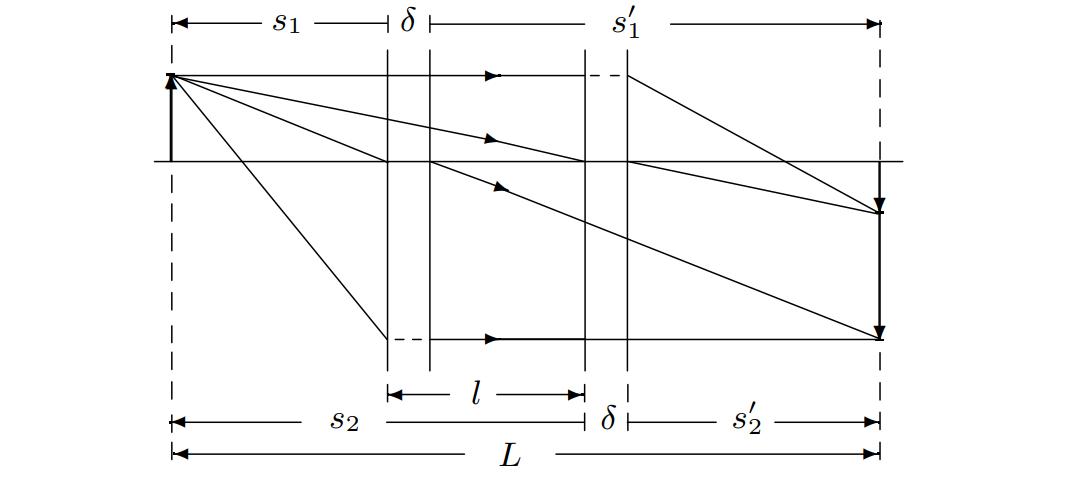
\includegraphics[width=0.8\linewidth]{Screenshot_2}
	\caption{Иллюстрация метода Бесселя}
	\label{3}
\end{figure}
Схема метода Бесселя для случая, когда $n = n'$ и $f' = -f$, представлена на \picref{3}. Тогда фокусное расстояние вычисляется по формуле:
\begin{equation}\label{Bessel}
	f = \frac{(L - \delta)^2 - l^2}{4(L-\delta)}.
\end{equation}

В данной работе предпочтение отдаётся методу Аббе.

\subsection{Определение фокусного расстояния тонкой собирающей линзы}

\paragraph{Способ 1.} Воспользуемся формулой тонкой линзы:
\begin{equation}\label{thin-lens}
	-\frac{1}{a}+\frac{1}{a'} = \frac{1}{f}.
\end{equation}
\paragraph{Способ 2.}
Фокусное расстояние тонкой собирающей линзы можно определить с помощью зрительной трубы, настроенной на бесконечность, то есть на параллельный пучок лучей. Разместив между предметом и зрительной трубой положительную линзу и перемещая её вдоль оси системы, можно найти резкое изображение предмета в окуляре зрительной трубы. При этом расстояние от середины линзы до предмета равно фокусному расстоянию тонкой линзы.

\subsection{Определение фокусного расстояния тонкой рассеивающей линзы}

\paragraph{Способ 1.} Сначала с помощью собирающей линзы получают на экране действительное изображение предмета $ S $ (точка $ S_1 $ на \picref{4}). Затем на пути лучей, выходящих из собирающей линзы, располагают исследуемую рассеивающую линзу и, отодвигая экран, получают чёткое изображение предмета на экране, образованное двумя линзами. Точка $ S_1 $ пересечения сходящихся лучей играет по отношению к рассеивающей линзе роль мнимого источника. Изображение источника переместится теперь в точку $ S_2 $. 

\begin{figure}[tbp]
	\centering
	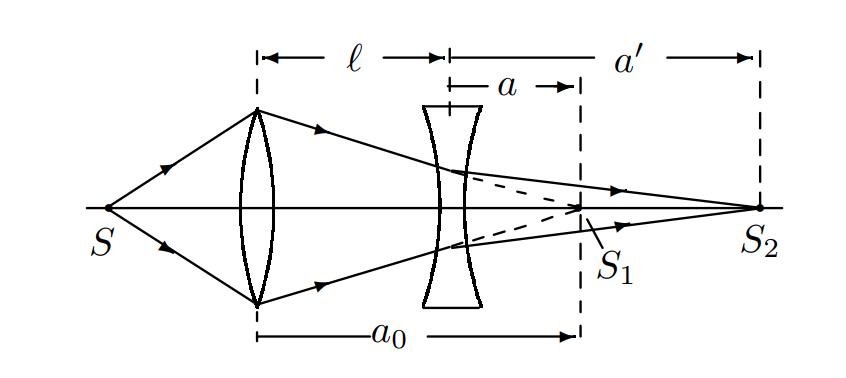
\includegraphics[width=0.8\linewidth]{Screenshot_5}
	\caption{Определение фокусного расстояния тонкой рассеивающей линзы}
	\label{4}
\end{figure}


Определив расстояния $ a = a_0 - l > 0$ и $ a'>0 $, рассчитывают фокусное расстояние рассеивающей линзы по формуле \eqref{thin-lens}.

\paragraph{Способ 2}

Если расстояние $ a $ на \picref{4} совпадает с модулем фокусного расстояния рассеивающей линзы, то изображение $S_2$ перемещается в бесконечность, то есть лучи выходят из линзы параллельным пучком. Параллельность пучка можно установить с помощью зрительной трубы, настроенной на бесконечность. Зная расстояние от первой линзы до точки $S_1$ и расстояние между линзами, нетрудно определить фокусное расстояние тонкой рассеивающей линзы. Для толстой отрицательной линзы этот метод позволяет определить только положение главного фокуса.


\subsection{Определение положения главных и фокальных плоскостей сложной оптической системы}

Для нахождения главных плоскостей системы недостаточно знать фокусное расстояние, нужно определить ещё положения главных фокусов. Это можно сделать при помощи зрительной трубы, настроенной на бесконечность. Отложив от главных фокусов отрезки, равные фокусному расстоянию, можно найти положения главных плоскостей системы. При этом необходимо учитывать возможность различного взаимного расположения кардинальных точек (плоскостей) сложной системы.


\section{Оборудование и инструментальные погрешности}

В работе используются:

\Equip{Линейка}{1}{\milli \metre}
\equip{Оптическая скамья с набором рейтеров}
\equip{Положительные и отрицательные линзы}
\equip{Экран}
\equip{Осветитель с ирисовой диафрагмой}
\equip{Зрительная труба}
\equip{Светофильтры}
\equip{Кольцевые диафрагмы}



\section{Результаты измерений и обработка данных}
\emph{Все измерения и расчёты в СИ.}

\subsection{Определение фокусных расстояний тонких линз при помощи экрана по методу Аббе}

\emph{Здесь и далее полагаем $ y = 10 \;мм $}

\label{abbe-1lens}
\paragraph{Линза 1.}

\begin{table}[h]
	\centering
	\begin{tabular}{|l|l|l|l|}
		\hline
		& $y'_1$, см & $x$, см & $x'$, см \\ \hline
		Опыт 1 & 8          & 199     & 132      \\ \hline
		Опыт 2 & 14         & 148     & 182      \\ \hline
		Опыт 3 & 41         & 100     & 453      \\ \hline
	\end{tabular}
	\caption{Серия опытов для 1 линзы по методу Аббе}
	\label{tab:1-abbe}
\end{table}


По формуле \eqref{abbe} рассчитаем $ f $. Посчитаем отдельно для изображения и для объекта (для минимизации погрешностей).

\begin{table}[h]
	\centering
	\begin{tabular}{|l|l|l|l|l|l|l|}
		\hline
		№       & 1  & 2  & 3   & 4  & 5  & 6   \\ \hline
		$f$, мм & 95 & 98 & 102 & 83 & 97 & 100 \\ \hline
	\end{tabular}
	\caption{Результат для 1 линзы}
	\label{tab:res1}
\end{table}

\begin{equation*}\label{key}
	f=96 \; мм.
\end{equation*}

На месте посчитаем погрешности. Инструментальные погрешности, посчитанные через Wolfram, составляют $ \delta = 9 $ мм, а случайные -- $ \sigma = 6 $ мм. То есть, по итогу,
\begin{equation*}\label{key}
	f=96\pm 10 \; мм.	
\end{equation*}

\paragraph{Линза 4.}

Получим действительное изображение от системы линз (\picref{4}). Из \eqref{thin-lens} получим:

\begin{equation*}\label{key}
	f= -75\pm 2\; мм.
\end{equation*}

\subsection{Определение фокусных расстояний тонких линз с помощью зрительной трубы}

\paragraph{Линза 1.}

С помощью зрительной трубы, определим, что:
\begin{equation*}\label{key}
	f_1 = 96\pm 3 \; мм,
\end{equation*}
\begin{equation*}\label{key}
	f_2 = 114\pm 3 \; мм.
\end{equation*}
Эти значения существенно отличаются, значит, линзу нельзя считать тонкой.

\paragraph{Линза 2.}

\begin{equation*}\label{key}
	f_1 = 134\pm 3\; мм,
\end{equation*}
\begin{equation*}\label{key}
	f_2 = 136\pm 3\; мм.
\end{equation*}
Так как в пределах погрешности, $ f_1 = f_2 $, то линзу 2 можно считать тонкой.

\paragraph{Линза 4.}

При $ a_0 = 283 \; мм $,
\begin{equation*}\label{key}
	f_1 = -70\pm 5 \; мм,
\end{equation*}
\begin{equation*}\label{key}
	f_2 = -75\pm 5 \;мм,
\end{equation*}
значит, линзу можно считать тонкой.

\subsection{Определение фокусных расстояний и положения главных и фокальных плоскостей сложной оптической системы}

Рассчитаем фокусное расстояние $ f_{2\Sigma} $.
Из формулы \eqref{abbe}, 
\begin{table}[h]
	\centering
	\begin{tabular}{|l|l|l|l|l|l|l|}
		\hline
		№       & 1  & 2  & 3  & 4  & 5  & 6    \\ \hline
		$f$, мм & 75 & 53 & 71 & 70 & 66 & 68 \\ \hline
	\end{tabular}
	\caption{Результат для системы линз по методу Аббе}
	\label{tab:res2}
\end{table}
\begin{equation*}\label{key}
	f_{2\Sigma} = 67 \pm 10 \; мм.
\end{equation*}
Погрешность определена так же, как в п. \ref{abbe-1lens}.

С помощью зрительной трубы найдём главные фокусы системы:
\begin{equation*}\label{key}
	F_{1\Sigma} = 38 \pm 3 \; мм,
\end{equation*}
\begin{equation*}\label{key}
	F_{2\Sigma} = 35 \pm 3 \; мм.
\end{equation*}

Построим чертёж на \picref{5}.

\begin{figure}[tbp]
	\centering
	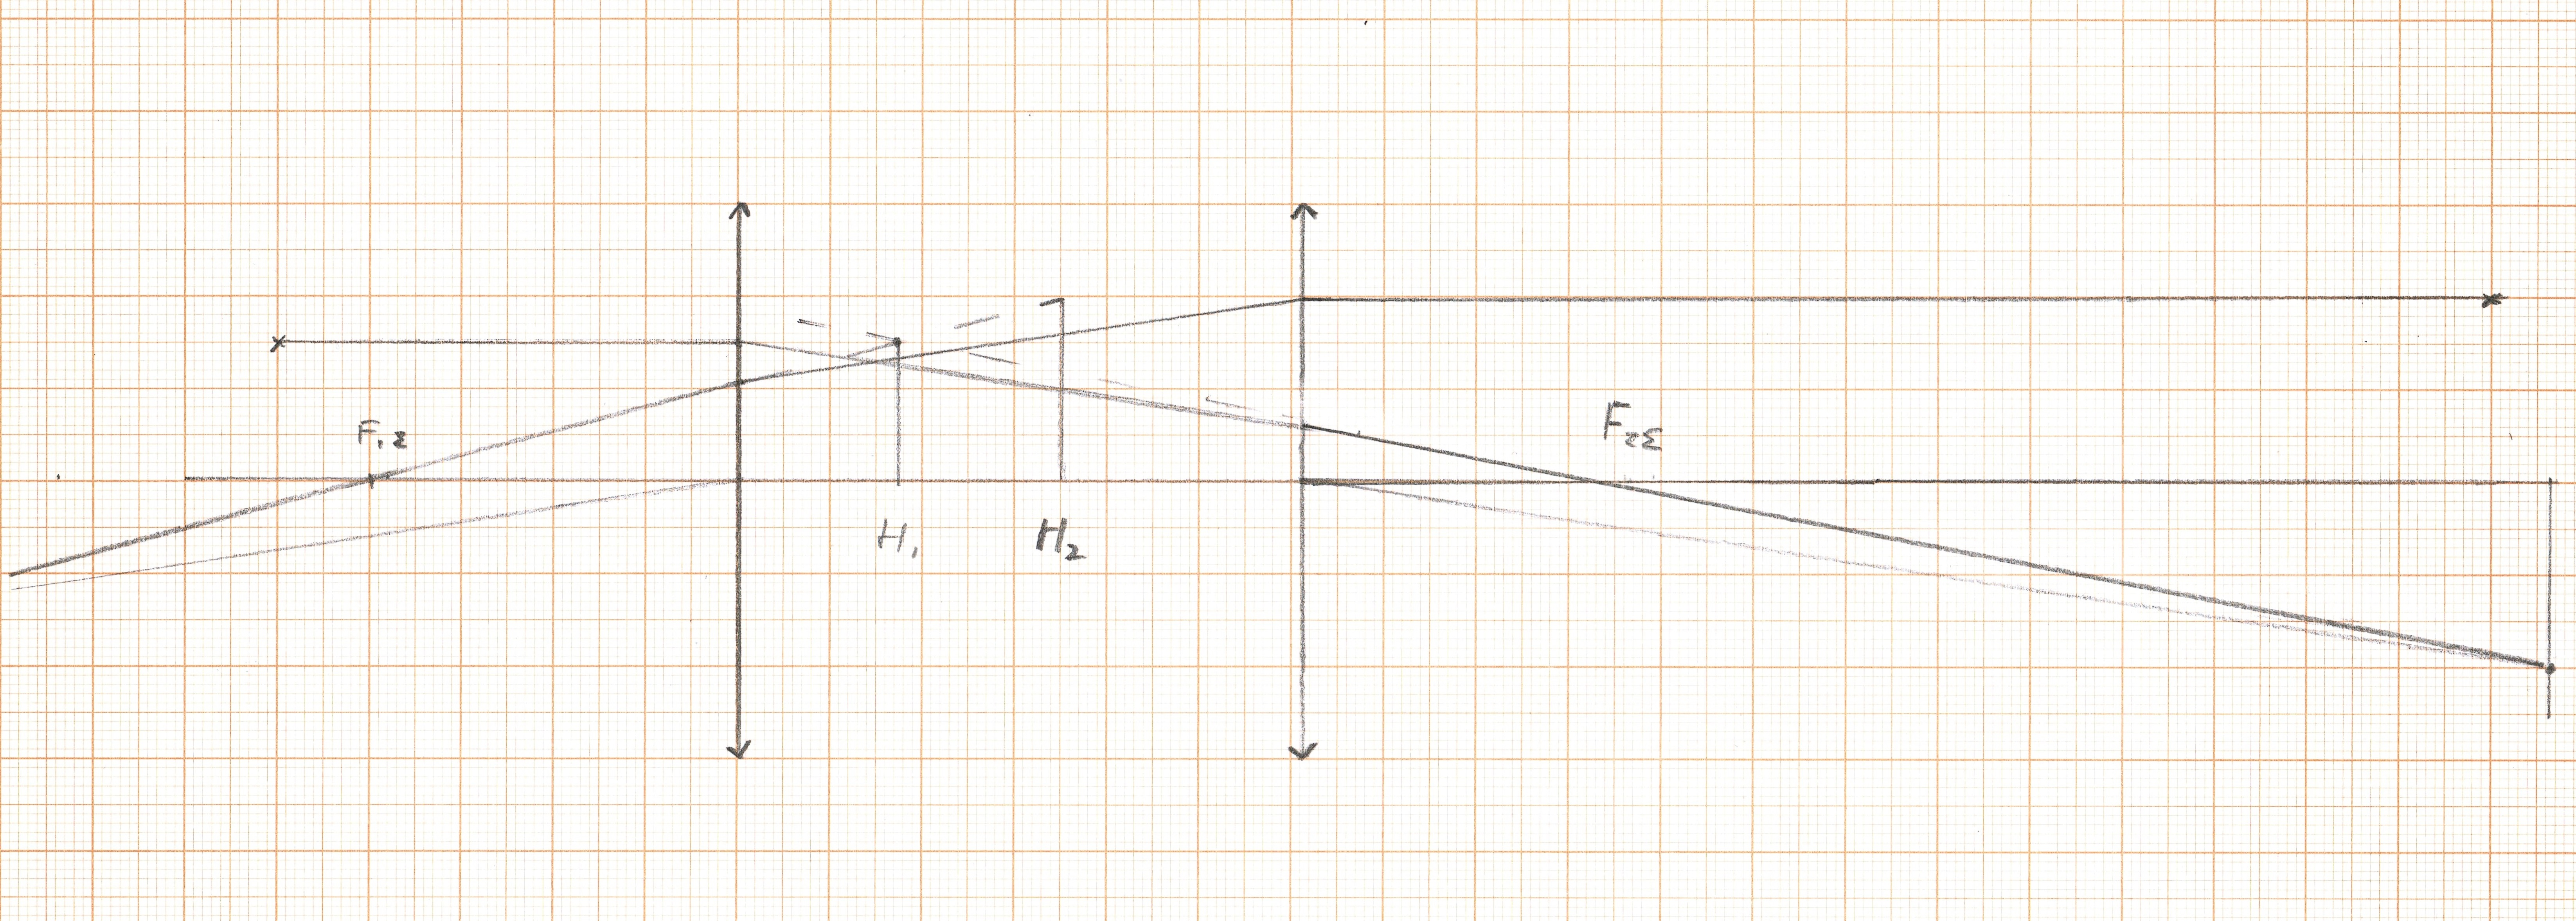
\includegraphics[width=\linewidth]{2021-02-17_085129}
	\caption{Определение параметров системы построением}
	\label{5}
\end{figure}


Согласно чертежу, 
\begin{equation*}\label{key}
	F_{1\Sigma} = 40\pm 1 \; мм,
\end{equation*}
\begin{equation*}\label{key}
	f_{1\Sigma} = 75\pm 1\; мм,	
\end{equation*}
\begin{equation*}\label{key}
	F_{2\Sigma} = 33\pm 1 \; мм,
\end{equation*}
\begin{equation*}\label{key}
	f_{2\Sigma} = 75\pm 1\; мм,
\end{equation*}
\subsection{Основные аберрации оптических систем}

\paragraph{Сферическая аберрация}

Нанесём на график (\picref{6}) зависимость $ -s (h^2) $, где $ h $ -- диаметр диафрагмы.
\begin{figure}[tbp]
	\centering
	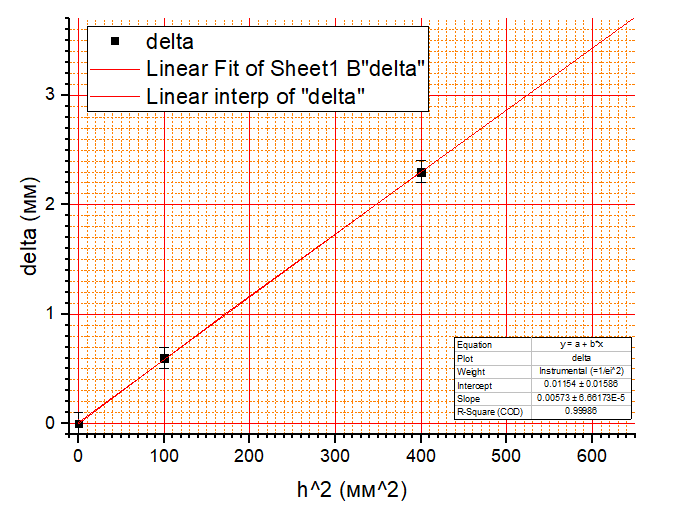
\includegraphics[width=0.8\linewidth]{Screenshot_7}
	\caption{Зависимость между разностями фокусного расстояния и диаметром диафрагмы}
	\label{6}
\end{figure}
Экстраполируя прямую до $ h^2 = 625 $, получим:
\begin{equation*}\label{key}
	\delta s (r) = 3.5\pm 0.2 \;мм.
\end{equation*}
Отсюда найдём показатель преломления: из формулы
\begin{equation}\label{key}
	\delta s (r) = \frac{1}{2} \left(\frac{n}{n-1}\right)^2 \frac{h^2}{f}
\end{equation}
следует:
\begin{equation}\label{key}
	n = \frac{2 f k+\sqrt{2} \sqrt{f} \sqrt{k}}{2 f k-1} = 1.5 \pm 0.1
\end{equation}
Такому показателю преломления соответствует оптическое стекло марки Крон.

\subsection{Хроматические аберрации}

Найдём хроматическую аберрацию линзы:

\begin{equation*}\label{key}
	\delta f_{хр} = 0.3 \pm 0.1 \; мм.
\end{equation*}

Эти данные не являются достаточно достоверными для определения по ним числа Аббе и марки стекла.

\subsection{Оценка погрешностей}

В п. \ref{abbe-1lens} и 4.3 формула инструментальных погрешностей вычислена в среде Wolfram Mathematica, затем сложена со случайной.

В п. 4.2 считаем погрешность линейки равной $ 3  $ мм, т. к. замер проведён недостаточно точно. 

В п. 4.4 ситуация осложняется недостаточной точностью инструмента и довольно несовершенным методом измерения, поэтому такая большая погрешность хроматических аберраций.

\section{Вывод}
Изучили несколько методов определения фокусных расстояний линз и сложных оптических систем. Провели исследование сферических и хроматических аберраций в линзах. Предположительно, мы имеем дело с оптическим стеклом марки Крон. 

\begin{thebibliography}{9}
	\bibitem{Siv} Сивухин Д. В. \emph{Общий курс физики. Том 4 Оптика}, 2004
	\bibitem{kir} Кириченко Н. А. \emph{Принципы оптики}, 2014
	\bibitem{max} \emph{Лабораторный практикум по общей физике. В 3 томах. Том 2. Оптика: учебное пособие} под ред. А. В. Максимычева
\end{thebibliography}
\end{document}